\documentclass[12pt]{article}
\usepackage{amsthm,amssymb,amsmath,amsfonts}
\usepackage[a4paper, top=25mm, bottom=30mm, left=25mm, right=25mm]{geometry}
\usepackage[pagebackref=false,colorlinks,linkcolor=black,citecolor=black]{hyperref}
\usepackage[nameinlink]{cleveref}
 \AtBeginDocument{%
    \crefname{equation}{برابری}{equations}%
    \crefname{chapter}{فصل}{chapters}%
    \crefname{section}{بخش}{sections}%
    \crefname{appendix}{پیوست}{appendices}%
    \crefname{enumi}{مورد}{items}%
    \crefname{footnote}{زیرنویس}{footnotes}%
    \crefname{figure}{شکل}{figures}%
    \crefname{table}{جدول}{tables}%
    \crefname{theorem}{قضیه}{theorems}%
    \crefname{lemma}{لم}{lemmas}%
    \crefname{corollary}{نتیجه}{corollaries}%
    \crefname{proposition}{گزاره}{propositions}%
    \crefname{definition}{تعریف}{definitions}%
    \crefname{result}{نتیجه}{results}%
    \crefname{example}{مثال}{examples}%
    \crefname{remark}{نکته}{remarks}%
    \crefname{note}{یادداشت}{notes}%
    \crefname{observation}{مشاهده}{observations}%
    \crefname{algorithm}{الگوریتم}{algorithms}%
    \crefname{cproof}{برهان}{cproofs}%
}

\usepackage{tikz}
\usepackage{graphicx}
\usepackage{color}

\usepackage{setspace}
\doublespacing

\usepackage{titletoc}
\usepackage{tocloft}
\usepackage{enumitem}

\usepackage{algorithm}
% \usepackage[noend]{algpseudocode}
\usepackage[noend]{algorithmic}
\renewcommand{\algorithmicrequire}{\textbf{Input:}}
\renewcommand{\algorithmicensure}{\textbf{Output:}}

\usepackage{tabularx}
\makeatletter
\newcommand{\multiline}[1]{%
  \begin{tabularx}{\dimexpr\linewidth-\ALG@thistlm}[t]{@{}X@{}}
    #1
  \end{tabularx}
}
\makeatother

\usepackage{float}
\usepackage{verbatim}
\makeindex
\usepackage{sectsty}
\usepackage{xepersian}
\SepMark{-}
\settextfont[Scale=1.2,Path=fonts/,BoldFont=B Nazanin Bold.ttf]{B Nazanin.ttf}
\setlatintextfont{Times New Roman}
\renewcommand{\labelitemi}{$\bullet$}

\theoremstyle{definition}
\newtheorem{definition}{تعریف}[section]
\newtheorem{remark}[definition]{نکته}
\newtheorem{note}[definition]{یادداشت}
\newtheorem{example}[definition]{نمونه}
\newtheorem{question}[definition]{سوال}
\newtheorem{remember}[definition]{یاداوری}
\newtheorem{observation}[definition]{مشاهده}
\theoremstyle{theorem}
\newtheorem{theorem}[definition]{قضیه}
\newtheorem{lemma}[definition]{لم}
\newtheorem{proposition}[definition]{گزاره}
\newtheorem{corollary}[definition]{نتیجه}
\newtheorem*{cproof}{برهان}



\begin{document}
\fontsize{12pt}{14pt}\selectfont

\begin{minipage}{0.1\textwidth}

\end{minipage}%
\hfill%
\begin{minipage}{0.6\textwidth}\centering
\fontsize{10pt}{10pt}\selectfont
به نام خداوند \\
تئوری یادگیری ماشین \\
دکتر سیدصالحی\\
جلسه سوم
 \\
\vspace{0.25cm}
\begingroup
\fontsize{8pt}{8pt}\selectfont
دانشکده ریاضی و علوم کامپیوتر \\
اسفند ماه 1402\\
\endgroup
\end{minipage}%
\hfill%
\begin{minipage}{0.1\textwidth}
\end{minipage}

\vspace{0.5cm}

\noindent\rule{\textwidth}{1pt}


\section*{$Neural\:Networks$}
مدل های اولیه ریاضیاتی که شکل گرفتند بر اساس عملکرد سلول های عصبی مغز انسان بودند.

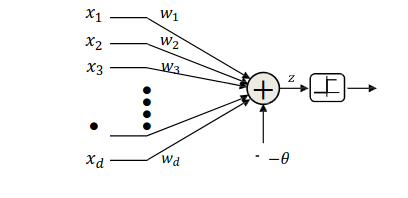
\includegraphics[width= 0.8\textwidth]{figs/model1.png}

پس از این مدل های اولیه طراحی دیگری پیش آمد که آستانه ای که میخواهند در نورون طراحی شده چک کنند را به شکل بایاس به نورون پاس بدهند و علامت نتیجه را به عنوان خروجی مطرح کنند.

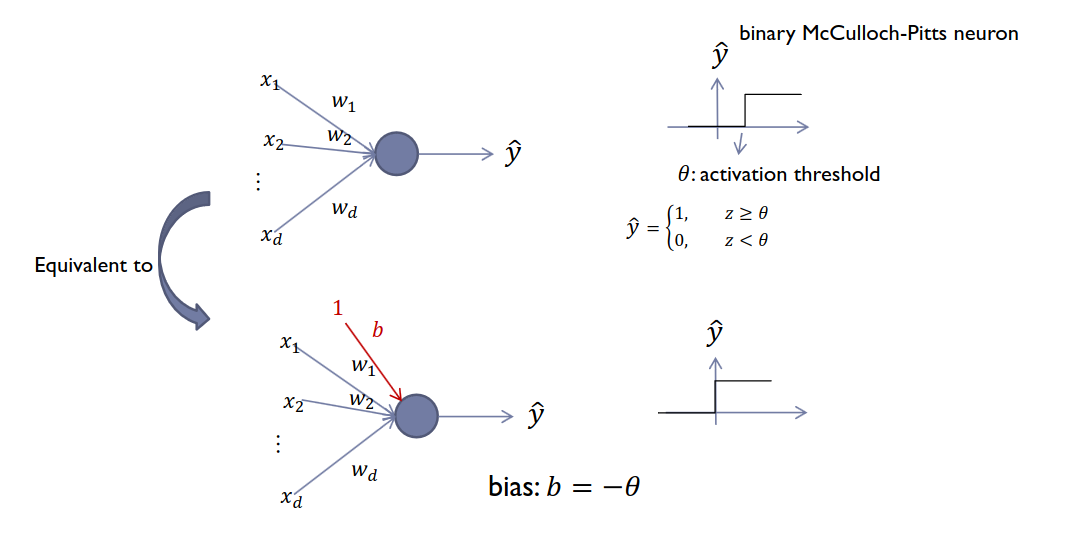
\includegraphics[width= 0.8\textwidth]{figs/model2.png}


این تغییر ما را به سمت طراحی مدل 
$perceptron$
میبرد. حال که مدل و فرم کلی این روش را میدانیم به سراغ الگوریتم یادگیری آن میرویم.
\subsection*{$learning\:algorithms$}
\subsubsection*{$perceptron$}

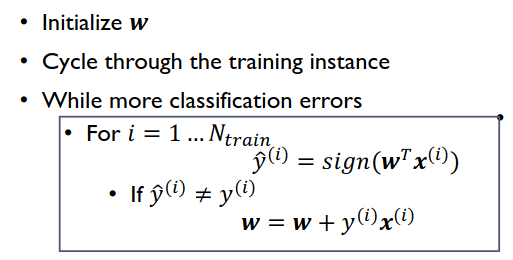
\includegraphics[width= 0.8\textwidth]{figs/perceptrion_la.png}

$update\:rule$

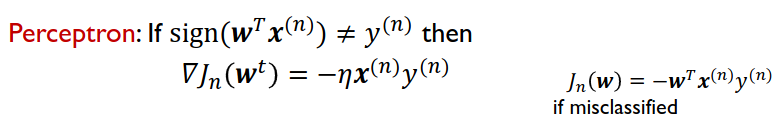
\includegraphics[width= 0.8\textwidth]{figs/perceptron_update_rule.png}


\subsubsection*{$ADALINE$}
$update\:rule$


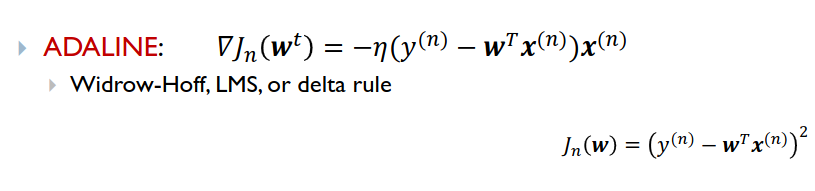
\includegraphics[width= 0.8\textwidth]{figs/adaline_update_rule.png}


یکی از راهکار های افزایش دقت مدل ها گسترش مدل ها با استفاده از اضافه کردن لایه های پنهان است.
اینجا با مفهوم 
$feed\:forward$
آشنا میشویم که دیتا ورودی را میگیرد و از لایه اول شروع میکند و همینطور لایه به لایه محاسبات را انجام میدهد و به خروجی ختم میشود. یکی از مدل های معروف این دسته از مدل ها 
$multi\:layer\:perceptron$
است.

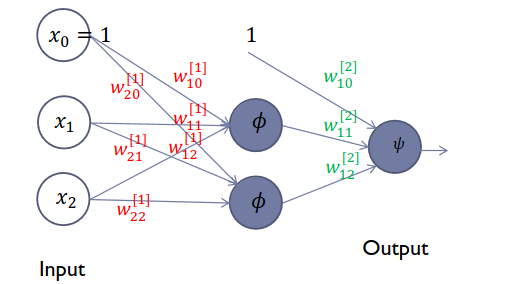
\includegraphics[width= 0.8\textwidth]{figs/MLP.png}


یکی از ویژگی های خوبی که ما را تشویق به استفاده از شبکه های عصبی میکند این است که هر لایه نمایانگر دسته ای از فیچر ها است و میتواند معنی دار باشد و ما از این اطلاعات بدست آمده در طول یادگیری میتوانیم استفاده کنیم.

\subsection*{$Sigmoid$}
عامل غیرخطی کننده ای که در مدل بالا میتوانید مشاهده کنید 
$activation\:function$
نام دارند که یکی از پرکاربردترین آنها تابع 
$sigmoid$
است.

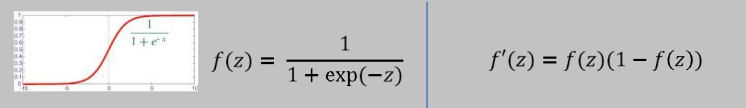
\includegraphics[width= 0.8\textwidth]{figs/sigmoid.png}


\subsection*{$BackPropagation$}
بیاید فرض کنیم که از روش 
$gradient\:descent$
برای اپدیت کردن پارامترها استفاده میکنیم. در این روش همانطور که به خاطر دارید به گرادیان نیاز داریم. اما پیچیدگی که در شبکه های عصبی داریم اینجاست که توابعی که در خروجی از نورون استفاده میکنیم در بحث مشتق پذیری دجار مشکل هستند و دیگر مساله بهینه کردن محسبات برای حساب گرادیان است.

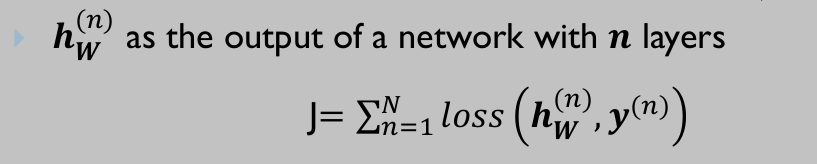
\includegraphics[width= 0.8\textwidth]{figs/img1.png}


و بنابر الگوریتم داریم 

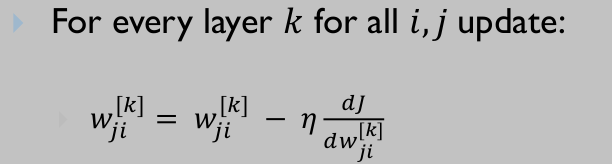
\includegraphics[width= 0.8\textwidth]{figs/img2.png}

تا هنگامی که 
$J$
همگرا شود.

\subsubsection*{$Chain\:Rule$}
قانونی است که در فرایند مشتق گیری و محاسبه گرادیان مورد استفاده قرار میگیرد.

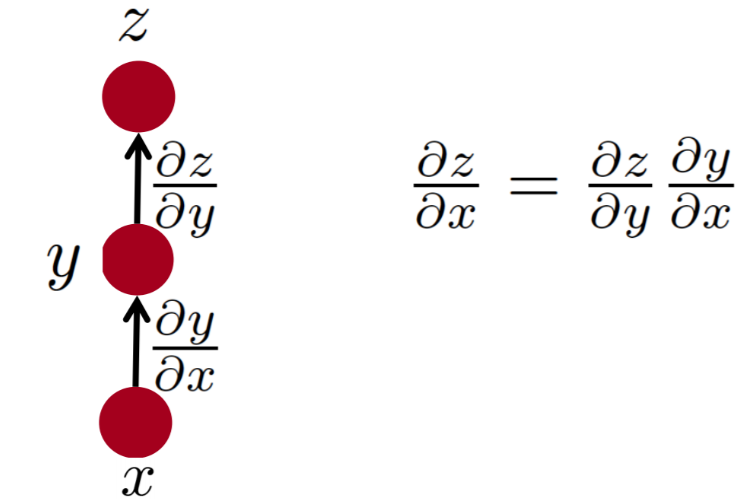
\includegraphics[width= 0.8\textwidth]{figs/chainRule.png}

اتفاقی که وقتی میخواهیم توی شبکه های عصبی مشتق بگیریم در یک نورون می افتد بدین شکل است.

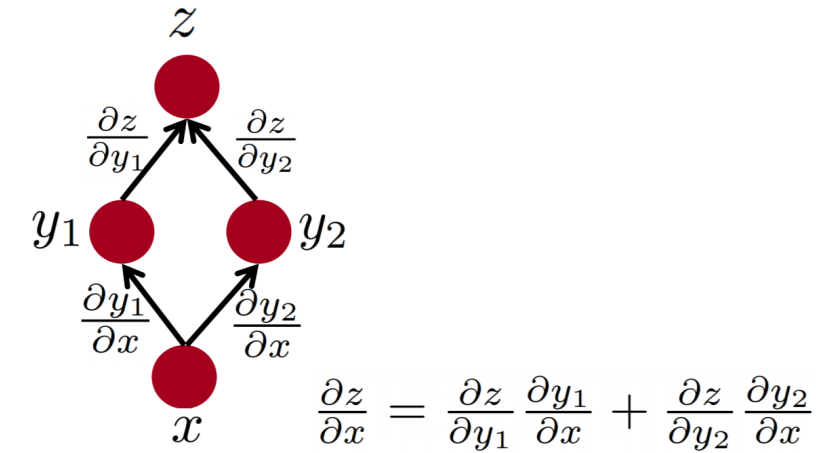
\includegraphics[width= 0.8\textwidth]{figs/multipath_chainrule.png}

چیزی که ما برای الگوریتممان نیاز داریم نحوه بدست آوردن 
\[
\frac{dJ}{dw_{ij}^{[k]}}
\]
است.

حال یک شبکه عصبی را در نظر بگیرید که 
$l - 1$
لایه نهان دارد. ورودی های این شبکه را به شکل 
$a^{[0]}$
نمایش میدهیم و خروجی آن را به فرمت 
$a^{[l]}$
معرفی میکنیم. 
تابع 
$f$
هم نمایانگر 
$activation\:function$
ها است.

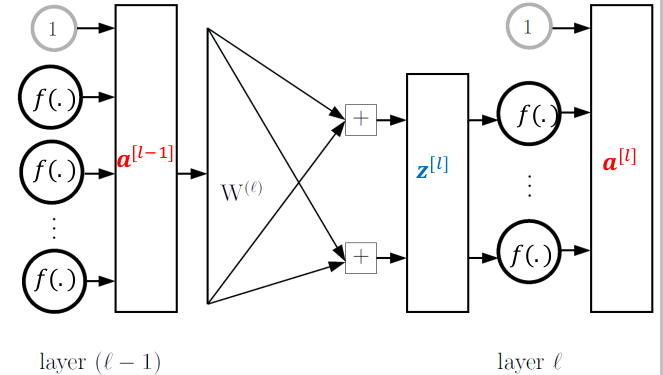
\includegraphics[width=0.8 \textwidth]{figs/img3.png}

حال طبق قاعده زنجیره ای داریم.

\[
\frac{\partial loss}{\partial w_{ji}^{[l]}} = \frac{\partial loss}{\partial a_{j}^{[l]}} \frac{\partial a_{j}^{[l]}}{\partial w_{ji}^{l}}
\]

مشتق خروجی نسبت به وزن های لایه اخر چیزی است که به راحتی با استفاده از مشتق 
$activation\:function$
و مشتق ورودی این تابع نسبت به وزن های این لایه محاسبه میشود.

\[
\frac{\partial a^{[l]}}{\partial w_{ji}^{[l]}} = f'(z_{j}^{[l]}) \frac{\partial z_{j}^{[l]}}{\partial w_{ji}^{l}} = f'(z_{j}^{[l]})a_{i}^{l - 1}
\]

پس در نهایت برای لایه اخر داریم.

\[
\frac{\partial loss}{\partial w_{ji}^{l}} = \frac{\partial loss}{\partial a_{j}^{[l]}} f'(z_{j}^{[l]}) a_{i}^{[l - 1]}
\]

و اما گرادیان گیری در لایه های قبلی آیا به راحتی لایه اخر است؟

\[
\frac{\partial loss}{\partial w_{ji}^{[l]}} = \frac{\partial loss}{\partial z_{j}^{[l]}} \frac{\partial z_{j}^{[l]}}{\partial w_{ji}^{[l]}} = \frac{\partial loss}{\partial z_{j}^{[l]}} a_{i}^{[l -1]}
\]

حال چگونه باید برای لایه های درونی این مشتق را بدست آورد؟

\[
\frac{\partial loss}{\partial z_{i}^{[l - 1]}}
\]

حال اگر از مواردی که بالاتر مطرح شد استفاده کنیم به این نتیجه میرسیم که برای محاسبه این مشتق نیازمند مشتق های لایه های بالاتر بصورت بازگشتی هستیم.

\[
\frac{\partial loss}{\partial z_{i}^{[l - 1]}} = \frac{\partial a_{i}^{[l - 1]}}{\partial z_{i}^{[l - 1]}} \Sigma_{j = 1}^{d^{[l]}} \frac{\partial loss}{\partial z_{j}^{[l]}} \times \frac{\partial z_{j}^{[l]}}{\partial a_{i}^{[l - 1]}}
\]

که نتیجتا داریم.

\[
= f'(z_{i}^{[l-1]}) \Sigma_{j = 1}^{d^{[l]}} \frac{\partial loss}{\partial z_{j}^{[l]}} \times w_{ji}^{[l]}
\]

حال که این روابط را بدست آوردیم به سراغ مفهوم 
$backpropagation$
میرویم.

\[
\frac{\partial loss}{\partial w_{ji}^{[l]}} = \frac{\partial loss}{\partial z_{j}^{[l]}} \times \frac{\partial z_{j}^{[l]}}{\partial w_{ji}^{[l]}}
\]

\[
= \delta_{j}^{[l]} \times a_{i}^{[l-1]}
\]

همانطور که در تصویر پایین هم میتوانید مشاهده کنید برای اینکه مشتق نسبت به یکی از وزن ها را بیابیم نیازمند اطلاعاتی از لایه های بالاتر نیاز داریم که سبب میشود تا ما مجبور باشیم برای محاسبه گرادیان یک مرحله 
$feedforward$
تا انتهای شبکه بریم و سپس از انتها شروع به مشتق گرفتن بکنیم که این عمل تحت عنوان 
$backpropagation$
شناخته میشود.

\[
\delta_{j}^{[l]} = \frac{\partial loss}{\partial z_{j}^{[l]}}
\]

\[
\delta_{i}^{[l-1]} = f'(z_{i}^{[l-1]}) \Sigma_{j=1}^{d^{[l]}} \delta_{j}^{[l]} \times w_{ji}^{[l]}
\]
\end{document}